\chapter{Software}

\section{STM32CubeMX}
The robot uses an STMicroelectronics STM32F446RE microcontroller (MCU) for low level sensor interfacing and motor control. Before starting the electrical design, the various hardware signals must be assigned to the MCU's GPIO with consideration for the device's peripherals such as timers and I\textsuperscript{2}C buses. STMIcroelectronics provides a program to this end called STM32CubeMX, shown in Figure \ref{fig:stm32cubemx}. Within the program, the user selects which MCU to configure and a graphical representation of the chip is shown on the GUI. The MCU's GPIO pins are arranged into banks of up to 16 pins each called ports. For example, PC2 is the second pin in Port C while PB11 is Pin 11 in Port B. The left column of the GUI lists the device peripherals including analog-to-digital converters (ADCs); various buses such as SPI, USART, and USB; and timers. Peripheral modes can be selected here such as USART mode (asynchronous, single-wire, LIN, etc) and flow control as well as timer clock sourcing and channel modes.

\begin{figure}[H]   % [h] means here
	\centering 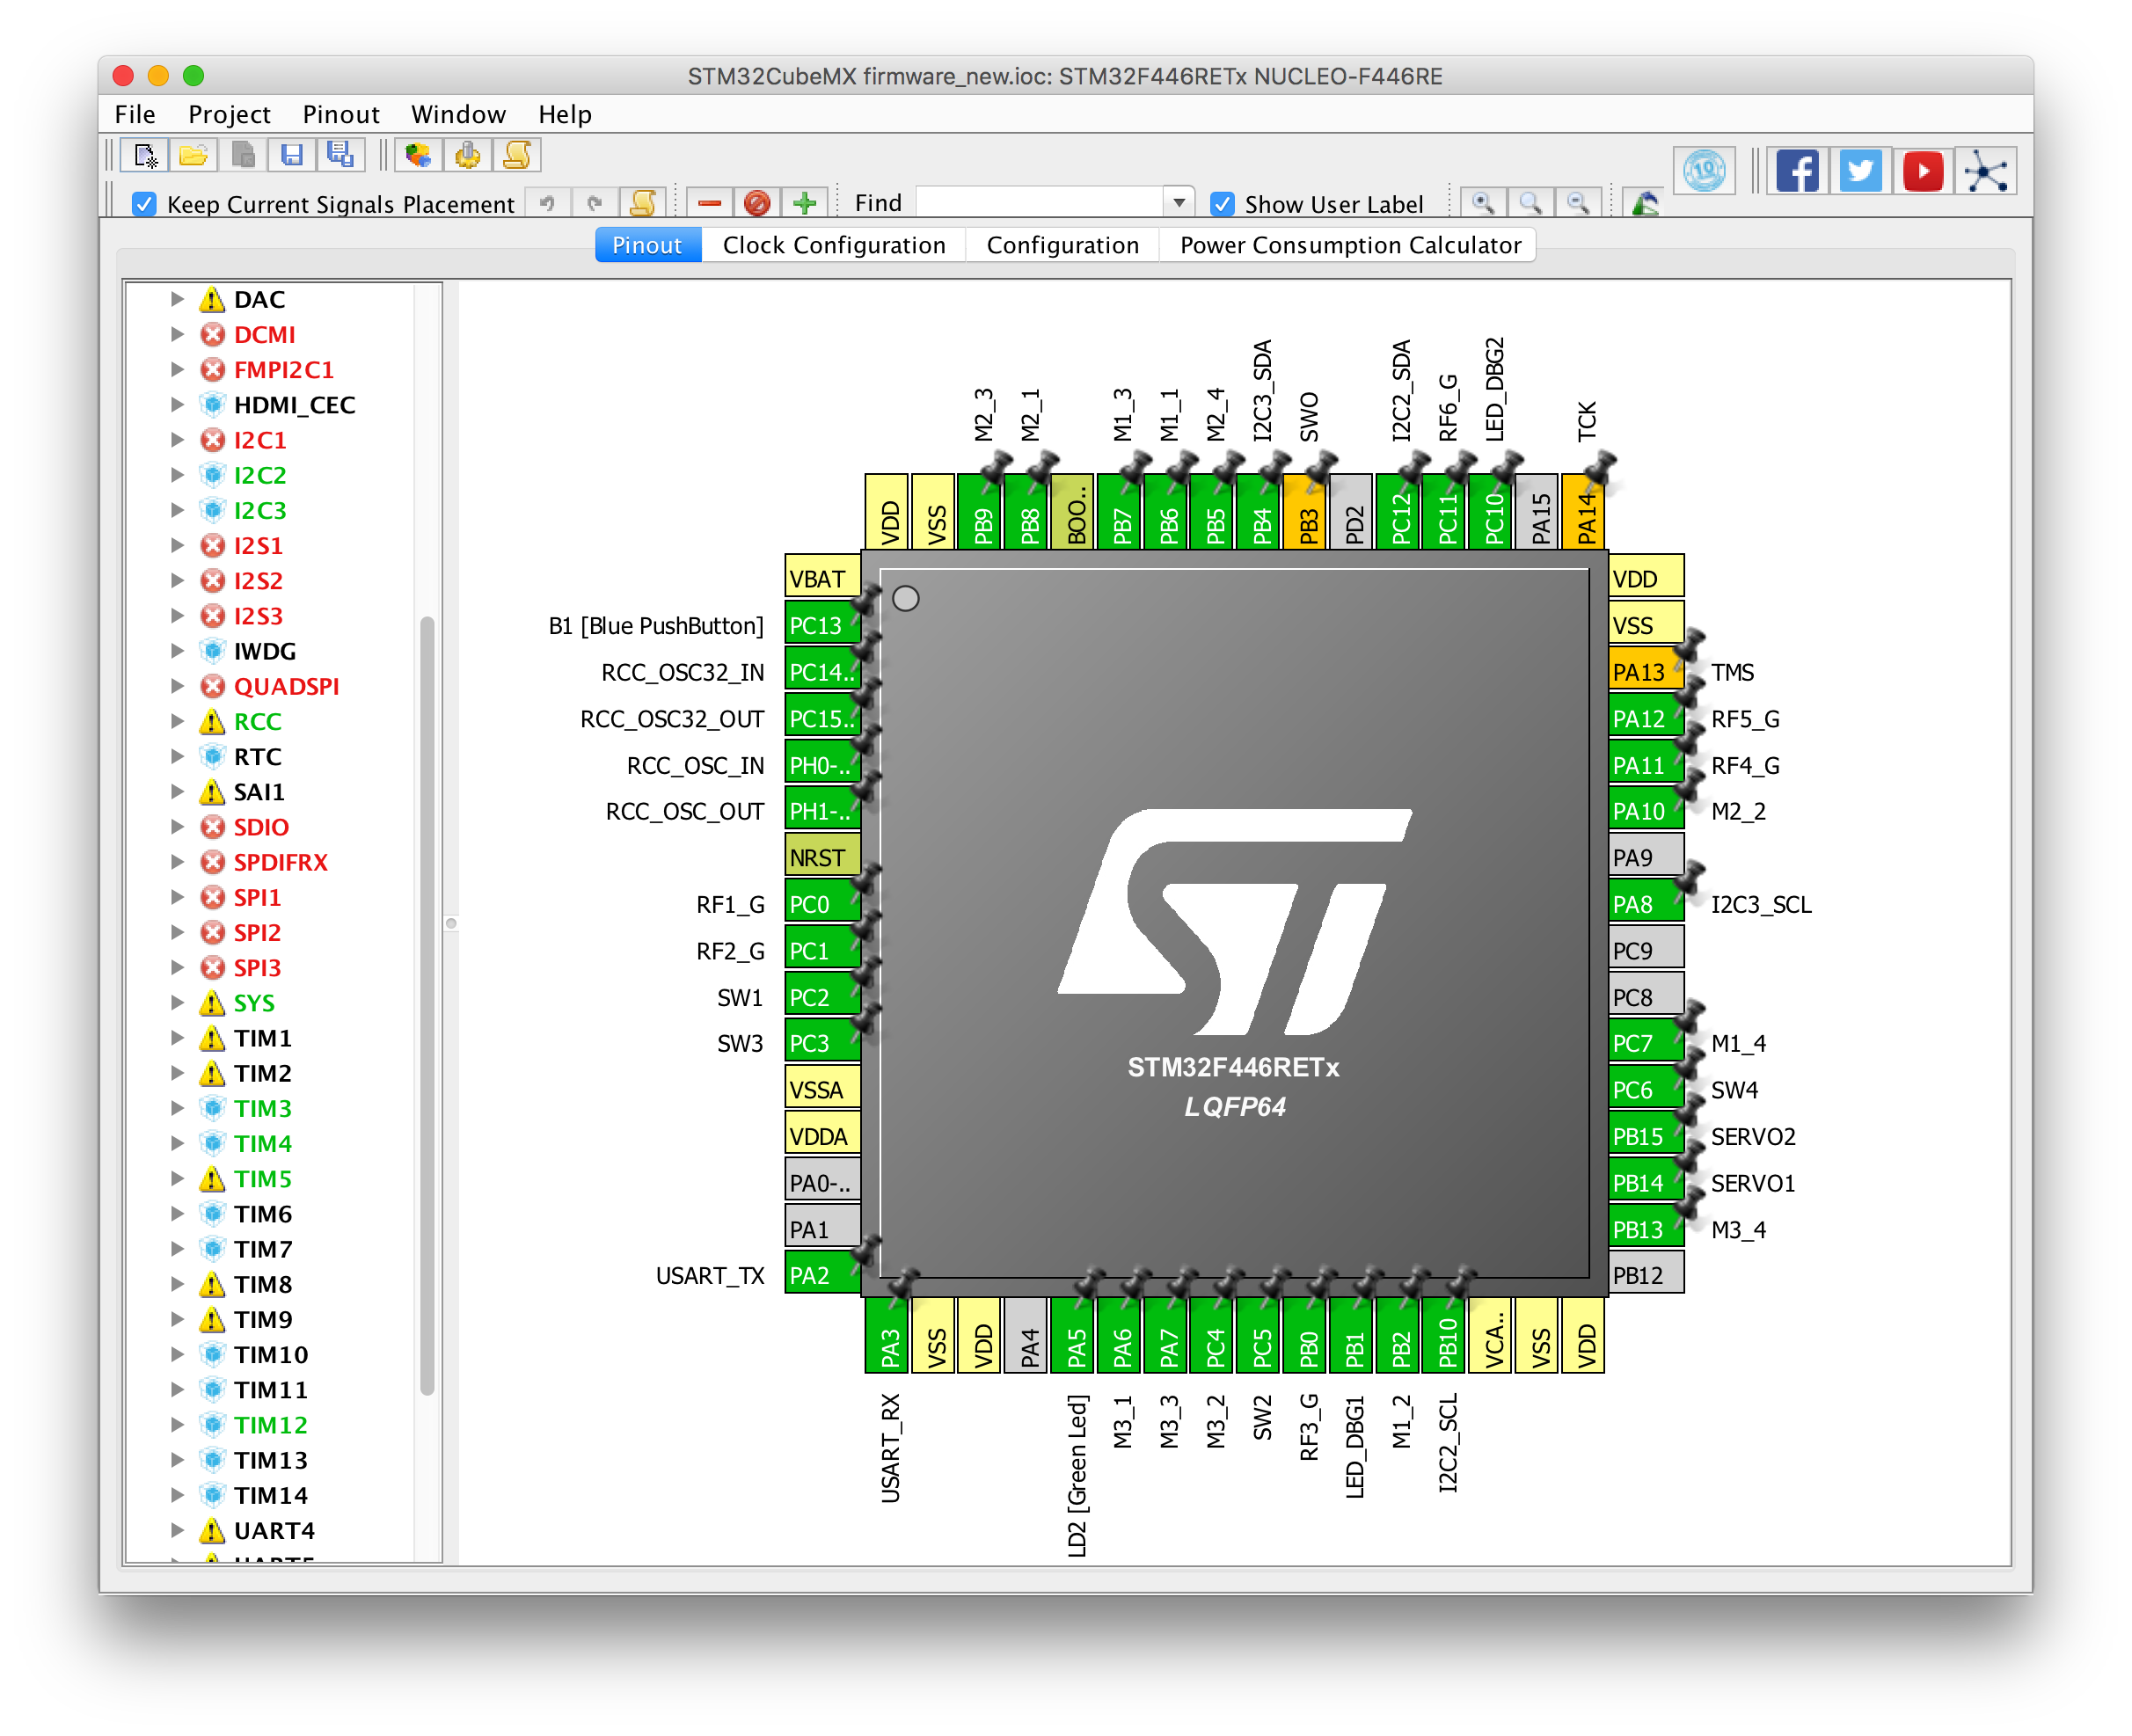
\includegraphics[width=6in, keepaspectratio]{figures/stm32cubemx.png}
	\caption{STM32CubeMX}\label{fig:stm32cubemx}
\end{figure}

The program greatly simplifies the puzzle-like process of pin assignment. Clicking a pin on the GUI brings up a menu of possible assignments. For example, clicking PB15, seen in Figure \ref{fig:stm32cubemx_pin}, shows that the pin can be used for the ADC, I2S2, as SPI2's MOSI, TIMER12's CH2 output, part of the USB differential data pair, as standard GPIO input or output, and more. As pins are assigned to various purposes, the true benefit of STM32CubeMX becomes clear. The program continually checks for compatibility issues and pin conflicts so pins can be iteratively assigned until errors are eliminated. For example, using a particular set of timers may actually prevent the use of I2C1 so either I2C2 or I2C3 must be used instead. This process is much faster and less error-prone than searching through the MCU's immense datasheet to manually check for assignment conflicts within every peripheral.

\begin{figure}[H]   % [h] means here
	\centering 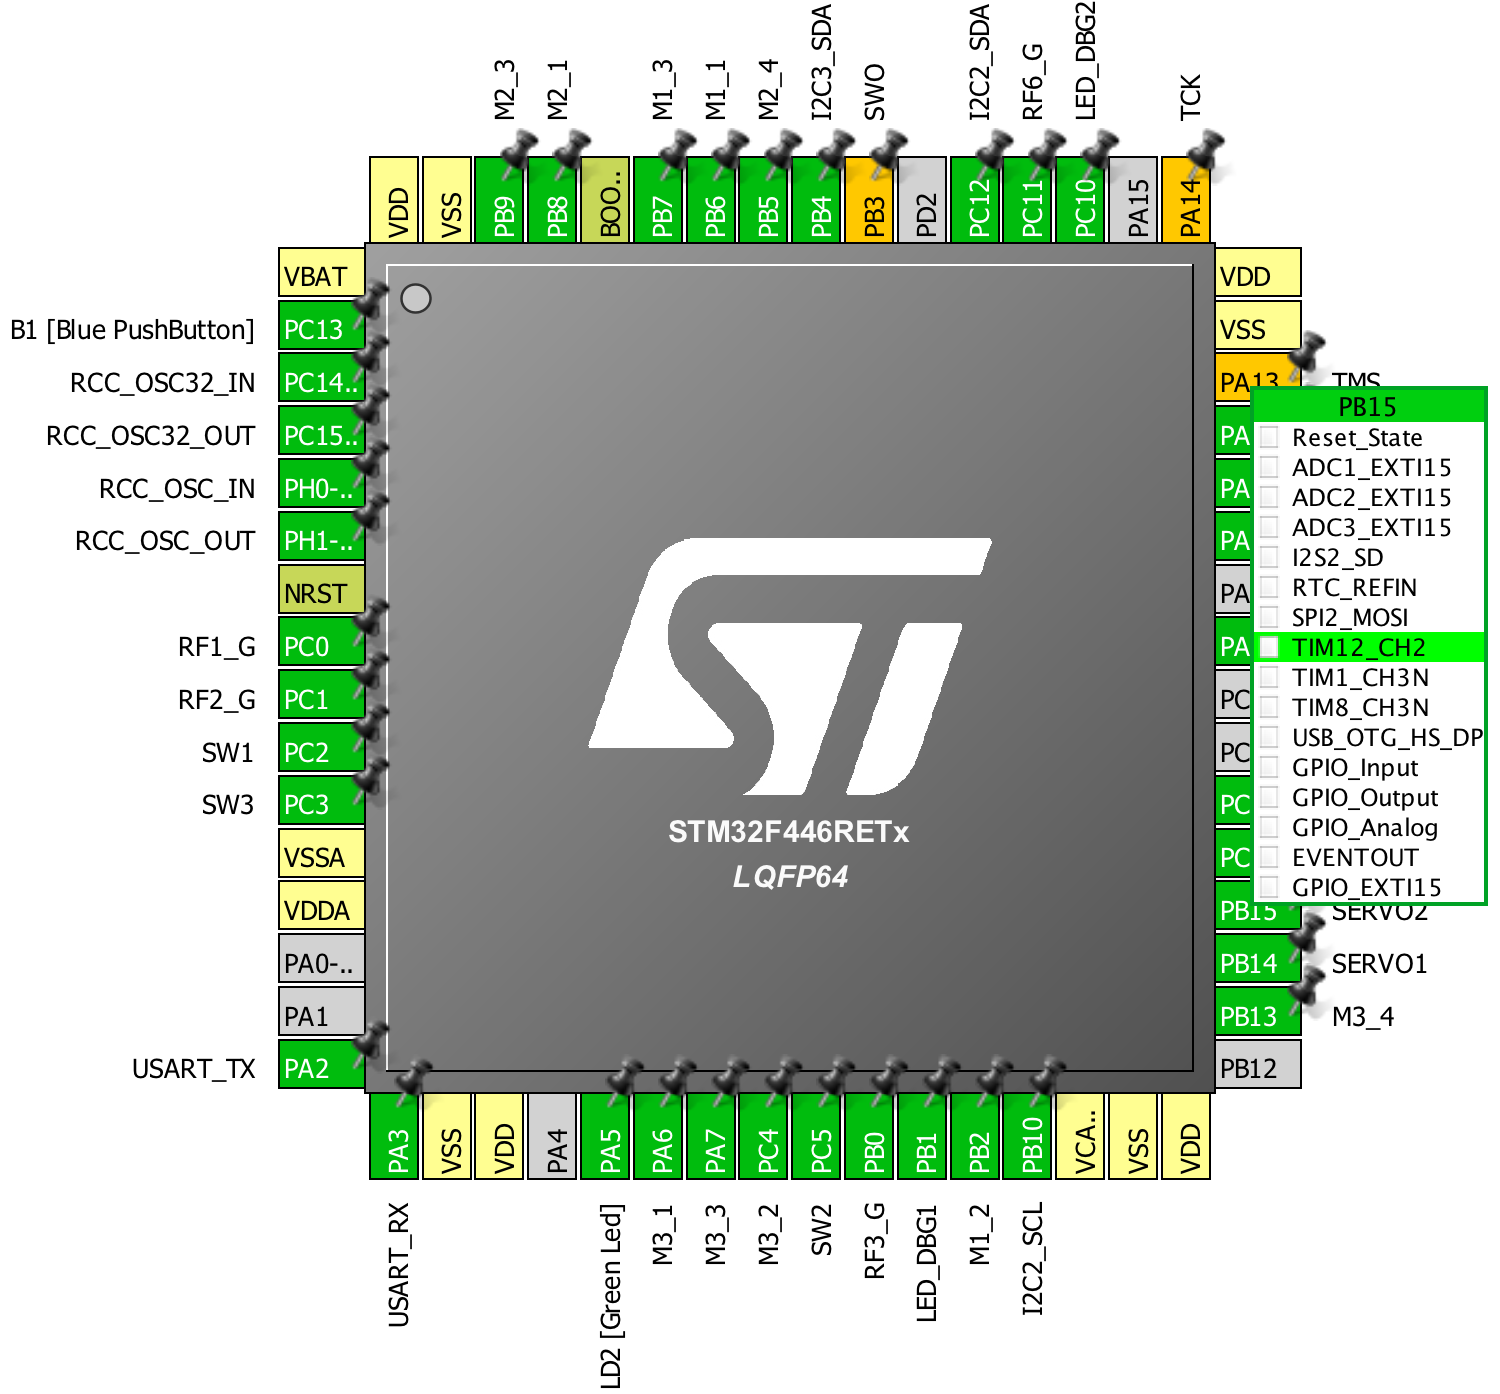
\includegraphics[width=6in, keepaspectratio]{figures/stm32cubemx_pin.png}
	\caption{STM32CubeMX -- Pin Menu}\label{fig:stm32cubemx_pin}
\end{figure}

The software also provides device-wide clock and PLL configuration as shown in Figure \ref{fig:stm32cubemx_clocks}. The MCU uses an external 8 MHz crystal to drive the internal PLL which then generates a 180 MHz system clock. Since the system is optimized for performance instead of power-saving, all advanced peripheral bus (APB) clocks are run at max frequency of 45 MHz for APB1 and 90 MHz for APB2. 

\begin{figure}[H]   % [h] means here
	\centering 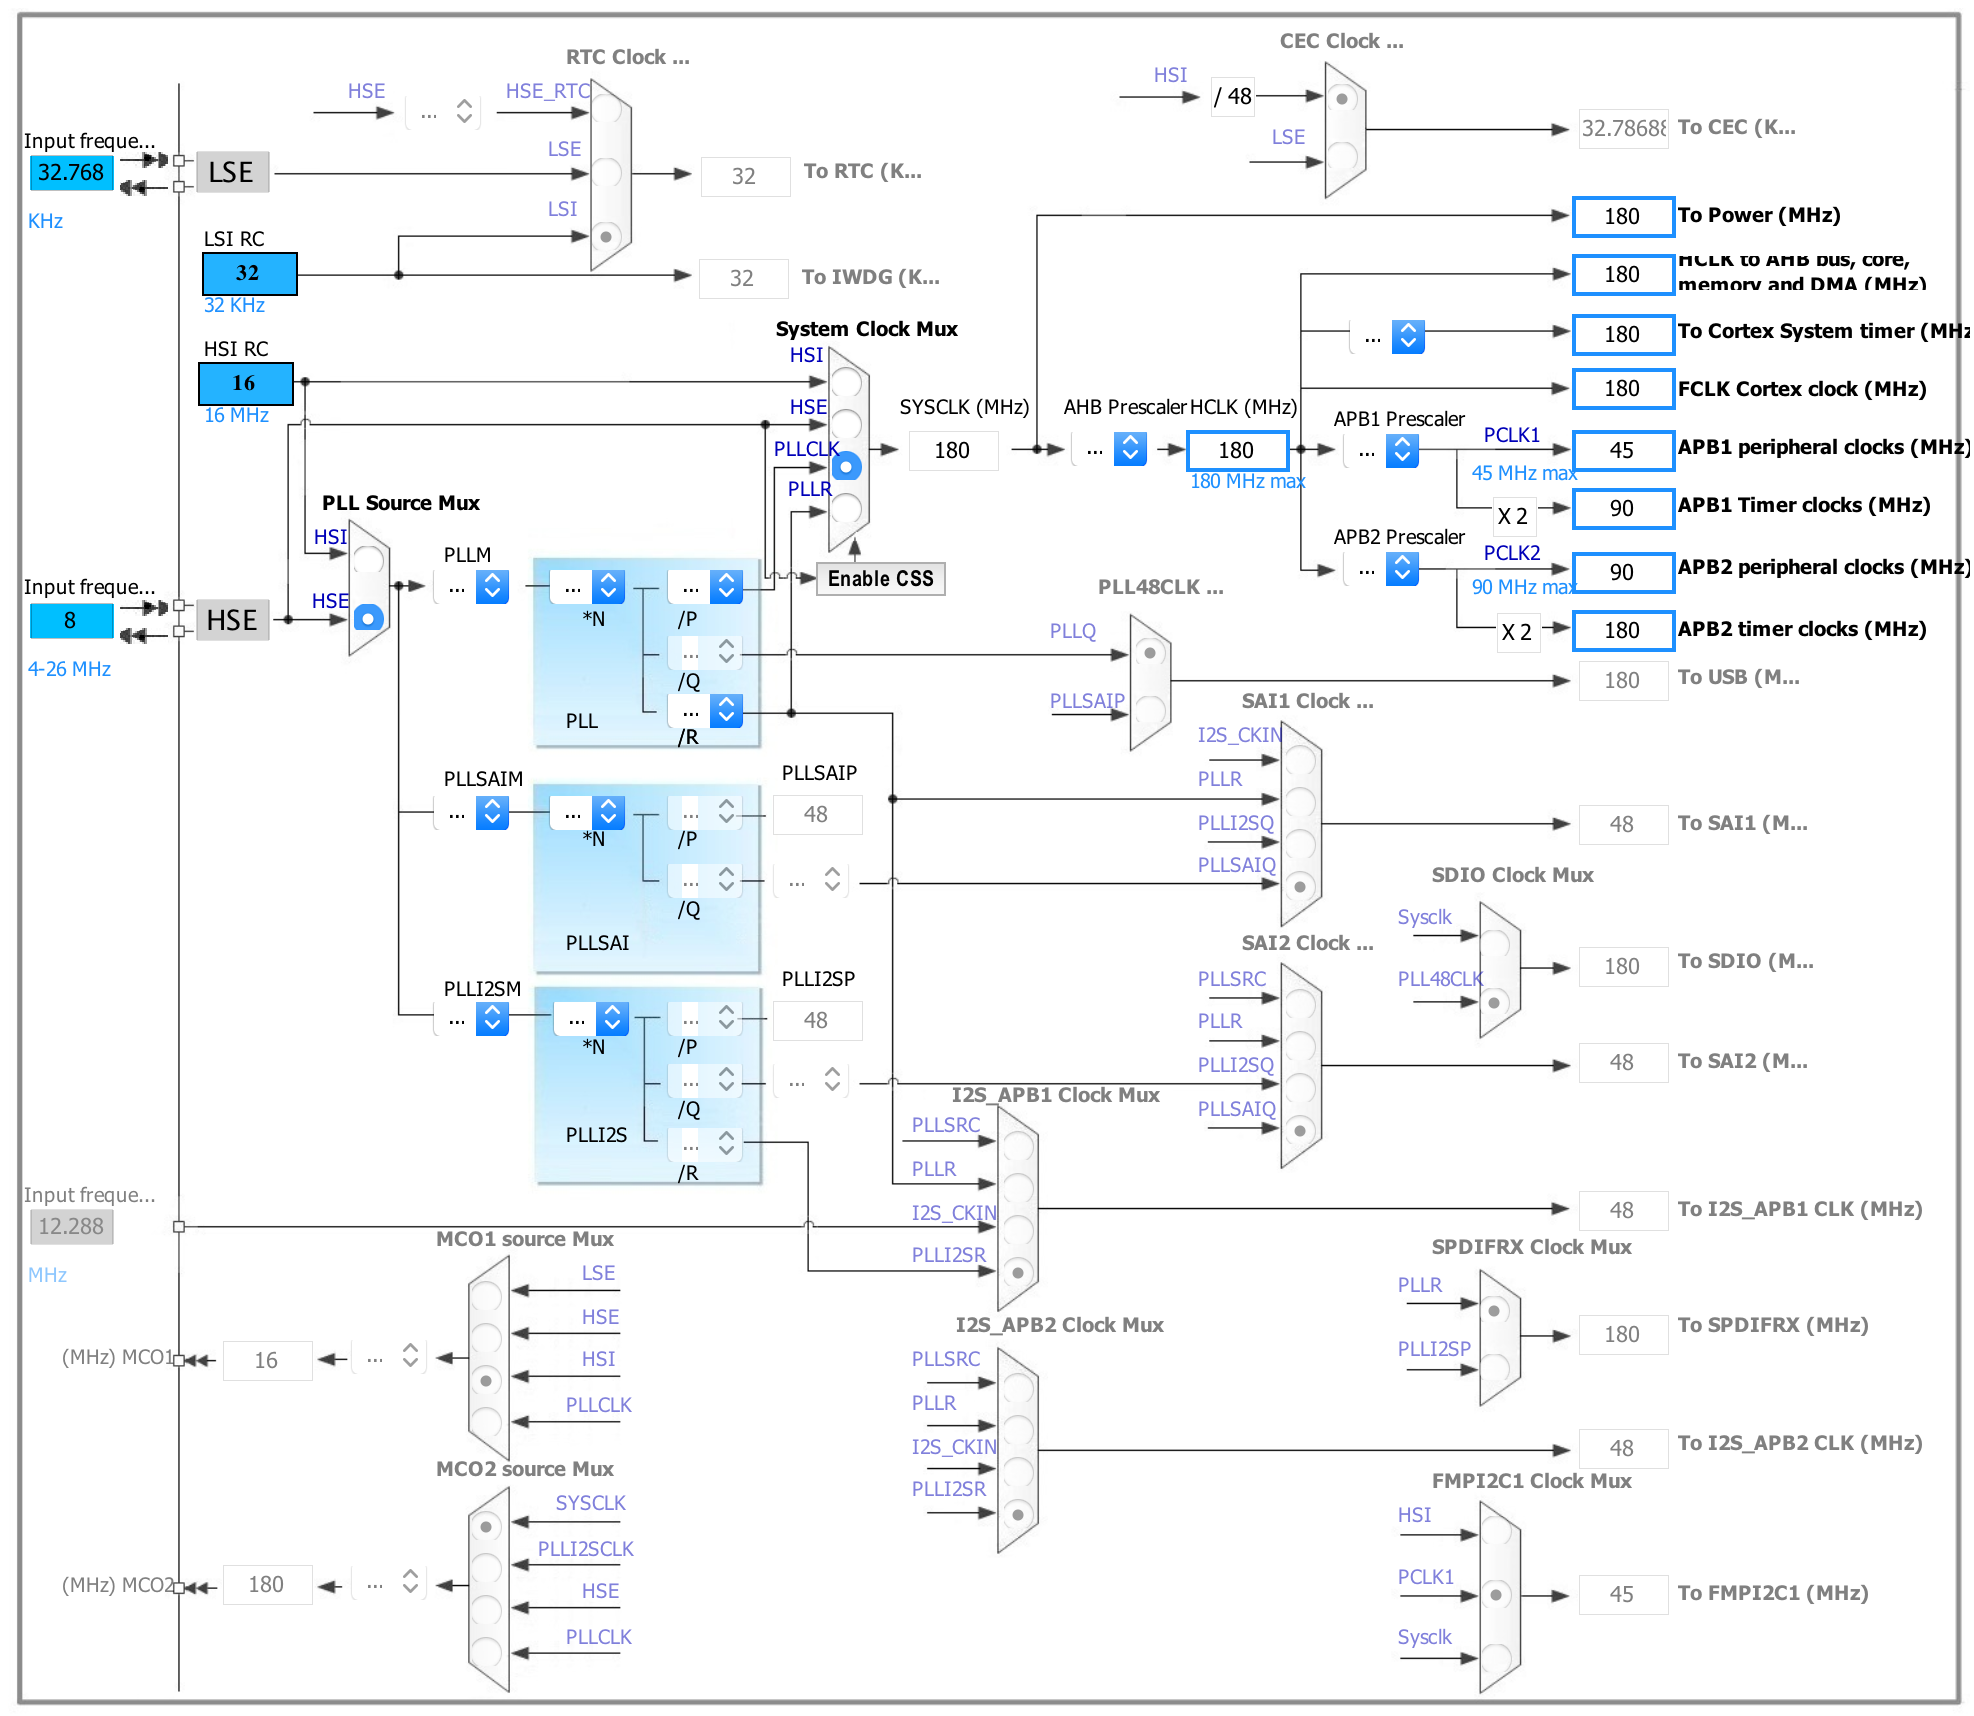
\includegraphics[width=6in, keepaspectratio]{figures/stm32cubemx_clocks.png}
	\caption{STM32CubeMX -- Clock Configurator}\label{fig:stm32cubemx_clocks}
\end{figure}

Another tab within STM32CubeMX provides detailed peripheral configuration. Both I\textsuperscript{2}C buses are set to 400 kHz with a 2:1 T\textsubscript{low}:T\textsubscript{high} duty cycle to meet the minimum pulse width requirement of slave devices. The USART peripheral is configured to 921,600 bits/s, 8-bit words, no parity, and one stop bit. The direct memory access (DMA) controller is set to process requests from the I\textsuperscript{2}C and UART peripherals to reduce processor load. 

The robot uses four of the MCU's timers: TIMER3, TIMER4, TIMER5, and TIMER12. Each of these timers sources its base clock from the APB1 clock which is 90 MHz. TIMER3 and TIMER4 output 6 PWM control signals for the motor drivers. They are set to count upward and reset after the counter reaches 2047 to produce a 43.9 kHz PWM frequency in the ultrasonic range. TIMER5, used for delay and timing functions, employs a clock prescaler of 9000 so the counter increases every 0.1 ms and never resets; the 32-bit counter has a maximum value of 4,294,967,295 corresponding to a counter rollover period of about 5 days. Finally, TIMER12 drives the PWM signals for servo control. It uses a 45 prescaler and a 50,000 counter period to produce a 40 Hz PWM frequency.

After configuring the various items above, STM32CubeMX can generate common boilerplate plate code to initialize and configure all the devices. Include and source files are generated on a by-peripheral basis to compartmentalize code. The program also generates a report of the device configuration, attached in Appendix \ref{appendix:stm32cubemx_report}.

\begin{figure}[H]   % [h] means here
	\centering 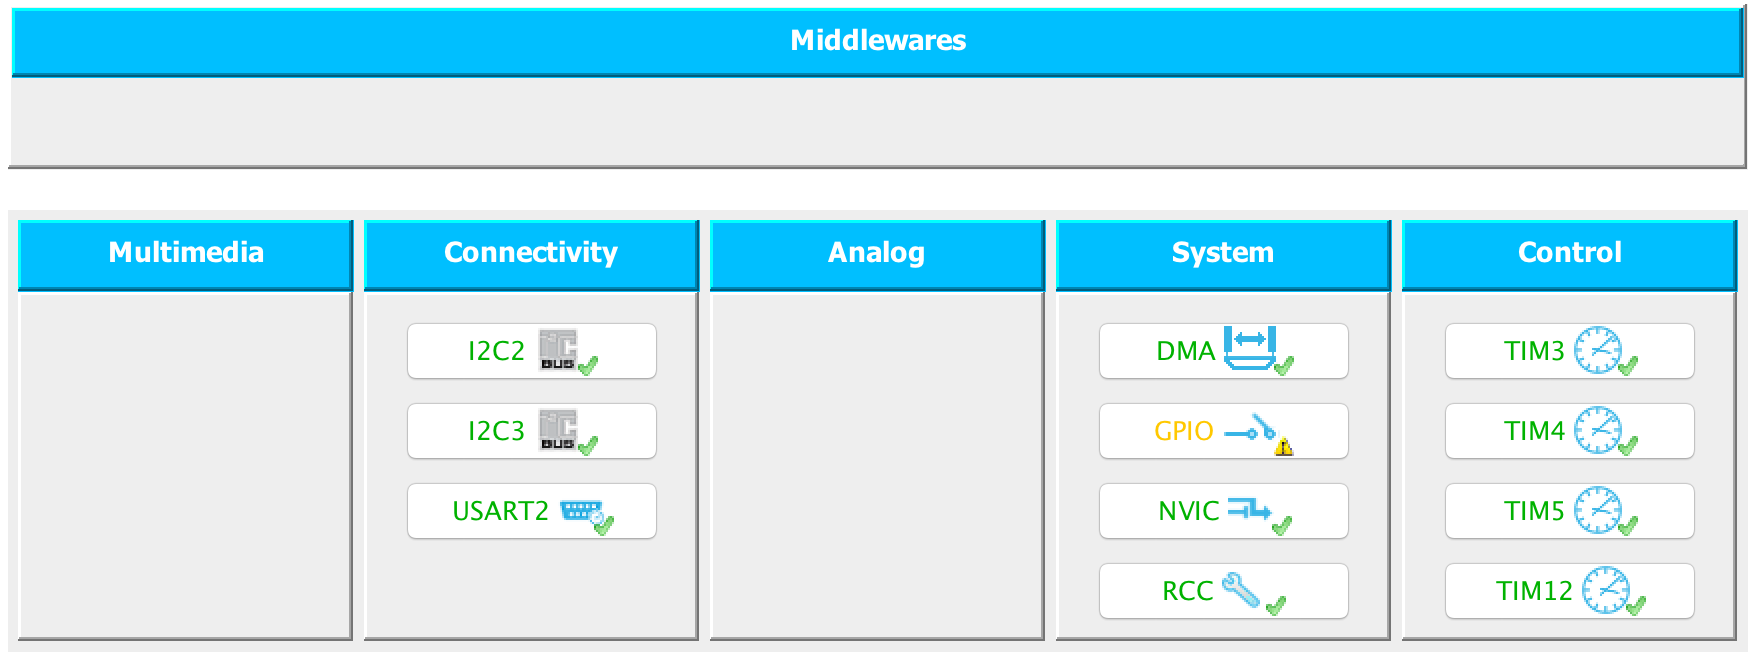
\includegraphics[width=6in, keepaspectratio]{figures/stm32cubemx_config.png}
	\caption{STM32CubeMX -- Peripheral Configurator}\label{fig:stm32cubemx_config}
\end{figure}

\section{Microcontroller Firmware}


\section{Definitions and Assumptions}
The robot is designed to only travel within a rectangular closed area of eight feet in the x direction and five feet in the y direction. The coordinate system is chosen as Cartesian with the origin placed at the bottom-left corner of the field. The position of the robot is always in the xy-plane since it cannot move vertically (z = 0). Therefore, $x$ refers to the robot position along the x-axis and ranges from 0 to 8 feet, and $y$ refers to position along the y-axis and ranges from 0 to 5 feet. Additionally, the robot can only rotate around the z-axis so $\theta$ refers to the angle of the robot in the xy-plane. Maintaining standard Cartesian coordinates, $\theta=\ang{0}$ is along the positive x direction while $\theta=\ang{90}$ is along the positive y direction.

\section{Kalman Filters}
The system relies on several different sensors to determine where it is within the environment, a problem commonly referred to as robot localization. The \textit{Kalman Filter} (KF), an optimal state estimator, performs noise filtering and sensor fusion, the process of combining measurements from multiple sensors. The filter operates on the principles of Bayesian inference and uses statistically noisy measurements over time and knowledge of the system to produce a more accurate estimate of an unknown variable than with measurement alone.

\subsection{Algorithm}
The Kalman Filter algorithm and equations are reproduced here from Roger Labbe's excellent interactive online book \cite{labbe_2017}.  The algorithm consists of two stages (not including initialization): prediction and update. During the first stage, the filter uses the current state and a process model (typically a function of time) to estimate the state in the next time step along with its uncertainty. The second stage uses sensor measurements to update the estimation by taking a weighted average based on the ratio of uncertainty between the prediction and measurement. 

\subsubsection*{Initialization}
Before the first run of the filter, initialize the estimated state (\textbf{x}, also called the posterior) and estimated state covariance matrix (\textbf{P}).
\subsubsection*{Predict}
During the predict phase, the process model is used to predict the future state (known as the prior) (\textbf{\=x}) after one time step by summing the posterior (\textbf{x}) multiplied by the \textit{state transition function} (\textbf{F}) with the control input model (\textbf{B}) multiplied by the control input (\textbf{u}). The covariance of prior (\textbf{\=P}) is larger than the posterior covariance (\textbf{P}) due to uncertainty in the process model (\textbf{Q}).
\begin{align*}
\bar{\textbf{x}} &= \textbf{Fx} + \textbf{Bu}\\
\bar{\textbf{P}} &= \textbf{FPF}^T + \textbf{Q}\\
\end{align*}

\subsubsection*{Update}
Make measurements (\textbf{z}, measurement mean) and determine their accuracy (\textbf{R}, measurement noise covariance). Calculate the residual (or difference) (\textbf{y}) between the measurement and the product of the measurement function (\textbf{H}) and the prior from the previous phase. \textbf{H} converts the prior from the state space to the measurement space. Calculate the weighting factor (\textbf{K}, Kalman gain), valued between 0 and 1, based on the whether the measurement or prior is more accurate. Set the new posterior, \textbf{x}, to an average of the measurement and prior, weighted by \textbf{K}. Finally, update the posterior's covariance, \textbf{P}, based on the measurement certainty. The algorithm then loops back to the predict phase using the newly-calculated posterior.
\begin{align*}
\textbf{y} &= \textbf{z} - \textbf{H}\bar{\textbf{x}}\\
\textbf{K} &= \bar{\textbf{P}}\textbf{H}^T(\textbf{H}\bar{\textbf{P}}\textbf{H}^T+\textbf{R})^{-1}\\
\textbf{x} &= \bar{\textbf{x}} + \textbf{Ky}\\
\textbf{P} &= (\textbf{I}-\textbf{KH})\bar{\textbf{P}}\\
\end{align*}

\subsection{Design}
The desired state variable \textbf{x} is chosen as the linear position, velocity, and acceleration in the x and y directions as well as the angular position, velocity, and acceleration about the z-axis:
\begin{align*}
\textbf{x} &= [x\ y\ \theta]^T\\
\dot{\textbf{x}} &= [\dot{x}\ \dot{y}\ \dot{\theta}]^T\\
\ddot{\textbf{x}} &= [\ddot{x}\ \ddot{y}\ \ddot{\theta}]^T\\
\end{align*}
The process model for position and velocity:
\[ \begin{cases} 
\bar{x}=x+\dot{x}\Delta t+0.5\ddot{x}(\Delta t)^2\\
\bar{\dot{x}}=\dot{x}+\ddot{x}\Delta t\\
\bar{\ddot{x}}=\ddot{x}\\
\end{cases} \]
Which can be written in the form:
\begin{align*}
\begin{bmatrix}\bar{x}\\ \bar{\dot{x}}\\ \bar{\ddot{x}} \end{bmatrix} &=
\begin{bmatrix}1 & \Delta t & 0.5(\Delta t)^2 \\
0 & 1 & \Delta t \\
0 & 0 & 1 \\\end{bmatrix}
\begin{bmatrix}x\\ \dot{x}\\ \ddot{x} \end{bmatrix}\\ 
\bar{\textbf{x}}&=\textbf{F}\textbf{x}
\end{align*}
The measurement vector is chosen as:
\[\textbf{z}=
\begin{bmatrix}z_x & z_{\ddot{x}} & z_y & z_{\ddot{y}} & z_{\theta} & z_{\dot{\theta}} \end{bmatrix}^T\]
The measurement noise matrix is shown below. The off-diagonals are 0 because the noise between sensors is assumed to be uncorrelated.
\[\textbf{R}=
\begin{bmatrix}\sigma^2_x & 0 & 0 & 0 &0 & 0\\
0 & \sigma^2_{\ddot{x}} & 0 & 0 & 0 & 0\\
0 & 0 & \sigma^2_y & 0 & 0 & 0 \\
0 & 0 & 0 & \sigma^2_{\ddot{y}} & 0 & 0\\
0 & 0 & 0 & 0 & \sigma^2_{\theta} & 0\\
0 & 0 & 0 & 0 & 0 & \sigma^2_{\dot{\theta}} \end{bmatrix}\]